%\documentclass[10pt,journal,final,letterpaper]{IEEEtran}
%\pdfpagewidth=8.5in
%\pdfpageheight=11in
%\documentclass[10pt,conference,letterpaper]{IEEEtran}
%\PassOptionsToPackage{pdfpagelabels=false}{hyperref} 
%\documentclass{acm_proc_article-sp}
\documentclass[5p]{elsarticle}

\usepackage[latin1]{inputenc}	% for Latin languages
\usepackage[T1]{fontenc}	% for ISO and UTF characters
\usepackage[english]{babel}	% for multilingual support
%\usepackage{hyperref}
%\hypersetup{
    %colorlinks=false,
%    pdfborder={0 0 0},
%}
\usepackage{graphicx}
\usepackage{multirow}
%\usepackage{stfloats}
\usepackage{booktabs}
%\usepackage[caption=false]{caption}
%\usepackage[caption=false,font=normalsize,labelfont=sf,textfont=sf]{subfig}
%\usepackage{color}
%\definecolor{Red}{rgb}{.9,0,0}
\usepackage{picins}


\newcommand{\fig}[4][htbp]{
  \begin{figure}[#1] {\centering\scalebox{#2}{\includegraphics{fig/#3}}\par}
    \caption{#4\label{#3}}
  \end{figure}
}

\newcommand{\multfigtwoh}[6][htbp]{
\begin{figure*}[#1]
  \centering
  \subfloat[]{\label{#3}\scalebox{#2}{\includegraphics{fig/#3}}}
  \subfloat[]{\label{#4}\scalebox{#2}{\includegraphics{fig/#4}}}
  \caption{#6}
  \label{#5}
\end{figure*}
}

\newcommand{\multfigtwov}[6][htbp]{
\begin{figure}[#1]
  \centering
  \subfloat[]{\label{#3}\scalebox{#2}{\includegraphics{fig/#3}}}\\
  \subfloat[]{\label{#4}\scalebox{#2}{\includegraphics{fig/#4}}}
  \caption{#6}
  \label{#5}
\end{figure}
}

\newcommand{\figR}[5][htbp]{
  \begin{figure}[#1]{\centering\scalebox{#2}{\includegraphics[angle=#5]{fig/#3}}\par}
    \caption{#4\label{#3}}
  \end{figure}
}

\newcommand{\figTC}[4][htbp]{
  \begin{figure*}[#1] {\centering\scalebox{#2}{\includegraphics{fig/#3}}\par}
    \caption{#4\label{#3}}
  \end{figure*}
}

\newcommand{\figEMPTY}[5][htbp]{
  \begin{figure}[#1]
    \fbox{\begin{minipage}{#2}\hfill\vspace{#3}\end{minipage}}
    \centering
     \label{#4}
    \caption{#5}
  \end{figure}
}

\newcommand{\tab}[3][htbp]{
  \begin{table}[#1]
    \footnotesize
    \centering
    \caption{#3}
    \include{tab/#2}
    \label{#2}
  \end{table}
}

\newcommand{\tabTC}[3][htbp]{
  \begin{table*}[#1]
    \footnotesize
    \centering
    \caption{#3}
    \include{tab/#2}
    \label{#2}
  \end{table*}
}

 %new commands 

%\setlength{\intextsep}{8pt}
%\setlength{\floatsep}{8pt}
%\setlength{\dblfloatsep}{8pt}
%\setlength{\abovecaptionskip}{3pt}
%\setlength{\belowcaptionskip}{1pt}
%\setlength{\intextsep}{-1ex} % remove extra space above and below in-line float
%Options    
%\floatsep - Space between floats. \dblfloatsep for 2 column format
%\intextsep - Space above and below in-line text floats
%\abovecaptionskip - Space above float caption
%\belowcaptionskip - Space below float caption

\hyphenation{Meta-pro-grams}

\journal{Journal of Systems Architecture}

\begin{document}

\begin{frontmatter}
    
%TODO find a more appropriate title
%A HLS-based framework for SoC design ??
%A portable C++ framework for hardware/software component communication
\title{A SoC platform supporting high-level synthesis for FPGAs}

%\author{Tiago Rog�rio M�ck and Ant�nio Augusto Fr�hlich\\
%\IEEEauthorblockA{Software/Hardware Integration Lab\\
%Federal University of Santa Catarina\\
%Florian�polis, Brazil\\ 
%Email: \{tiago,guto\}@lisha.ufsc.br}
%}

%ACM stuff
%\numberofauthors{2}
%\author{
  %\alignauthor
  %Tiago Rog�rio M�ck
  %\alignauthor
  %Ant�nio Augusto Fr�hlich
  %\and\alignauthor
  %\affaddr{Software/Hardware Integration Lab}\\
  %\affaddr{Federal University of Santa Catarina}\\
  %\affaddr{Florian�polis, Brazil}
  %\email{\{tiago,guto\}@lisha.ufsc.br}
%}
%\author{
  %\alignauthor
  %\and
  %\alignauthor
  %\and
  %\alignauthor
  %Authors omitted for blind review
%}

%Elsevier
\author{Tiago Rog�rio M�ck\corref{cor1}\fnref{fn1}}
\ead{tiago@lisha.ufsc.br}
\author{Ant�nio Augusto Fr�hlich\fnref{fn1}}
\ead{guto@lisha.ufsc.br}
\address{Federal University of Santa Catarina, Florian�polis, Brazil}

\cortext[cor1]{Corresponding author}

\fntext[fn1]{Authors full address:\\
UFSC/CTC/LISHA\\
PO Box 476\\
88040-900 Florian�polis - SC - Brazil\\
Phone/Fax: +55 48 3721-9516 }

%ACM / IEEE
%\maketitle

%TODO write a more appropriate abstract
\begin{abstract}
With the gradual increase in the complexity of \textit{System-on-Chip}~(SoC) designs, system-level
approaches that leverage on \textit{high-level synthesis}~(HLS) techniques are becoming the
workhorse of current SoC design flows. In this scenario, we propose a flexible FPGA-based SoC
platform for the deployment of SoCs in a HLS-capable environment. The proposed hardware/software
infrastructure relies on a \textit{Network-on-Chip}-based architecture to provide transparent
communication mechanisms for hardware and software components. We verify the performance and area
footprint of our communication infrastructure through the implementation of a SoC for digital
PABX systems.
\end{abstract}

%\begin{IEEEkeywords}
%FPGA; System-on-chip; System-level design; High-level synthesis; HW/SW co-design;
%\end{IEEEkeywords}

%ACM
%\category{B.6.3}{LOGIC DESIGN}{Design Aids}[Automatic synthesis]
%\terms{Design, Languages}
%\keywords{FPGA, System-on-chip, System-level design, High-level synthesis, HW/SW co-design}

%Elsevier
\begin{keyword}
FPGA \sep System-on-chip \sep System-level design \sep High-level synthesis \sep HW/SW co-design
\end{keyword}

\end{frontmatter}

%TODO throughout the paper, must establish better what is the platform, the architecture and the
%framework. Must avoid confusion using this terms.

%TODO Adicionar um se��o descrevevndo o tratamento da semantica e da convers�o de tipos de dados
%     entre hardware e software (usando o serializer)

%TODO Novo case ?? Detector de DTMA com suporte a multiplos canais. Aloca os core DTMF e os
%     buffers para os frames dinamicamente (usando o static alloc em hardware) a medida que for
%     necess�rio. Se o n� de buffers > n� de cores, ent�o multiplexa os cores 


\section{Introduction}
\label{sec:introduction}      
\textit{System-on-Chip}~(SoC) design are becoming more sophisticated as the advances of
the semiconductor industry allows the use of an increasingly amount of computation resources in a
wide range of applications. Low-power and small \textit{field-programmable gate arrays}~(FPGAs) now
reaching the market are one of the products of these advances, enabling the rapid deployment of
complex and fully customized SoC designs even for small-scale applications. In this scenario, the
strict time-to-market requirements of most applications demands a better productivity than what is
possible with current \textit{register transfer level}~(RTL) methodologies, thus leading to a
growing demand for \textit{high-level synthesis}~(HLS) solutions.

Also known as \textit{electronic system-level}~(ESL) synthesis, HLS is a (semi-)automatic process
that creates cycle-accurate RTL specifications from untimed or partially timed behavioral
specifications. Current \textit{electronic design
automation} (EDA) \cite{Calypto:Catapult,Xilinx:AutoESL} tools already support hardware synthesis
from high-level C++ and SystemC descriptions, enabling the use of higher-level implementation
techniques, such as \textit{object-oriented programming}~(OOP). Several works have already
demonstrated the applicability of HLS for implementing computational-intensive hardware
accelerators~\cite{Fingeroff:2010} and the use of HLS solutions in FPGA design
flows~\cite{Cong:2011}.

%maybe remove this ?
%\figSC{.57}{fig_full_flow}{Generic HLS-based SoC design flow}
%Figure~\ref{fig_full_flow} gives an overview of a generic SoC implementation flow considering HLS.

Such design flows consist in a set of basic steps. The developer provides high-level
implementations (usually in C++-based languages) of the software and hardware components that build
up the application.  In the software side of the flow, the components are compiled and usually
linked with a run-time support system, such as a \textit{real-time operating system}~(RTOS). The
product of the software flow is a set of binaries for one or more \textit{instruction-set
architectures}~(ISA) (e.g. in a \textit{Multiprocessor SoC}~(MPSoC) with heterogeneous processors).
The hardware implementation flow is more complex and encompass a process which includes: 1)
C++-to-RTL synthesis using a HLS tool; 2) binding of the generated RTL descriptions with a set of
existing \textit{intellectual properties}~(IPs) (e.g. soft-processors, IO devices, memories,
interconnection) in order to build a hardware platform; and 3) synthesis of the final platform to
the target FPGA device.

%Apart from the physical platform, high-level hardware simulation models of the input components
%and IPs may be generated and assembled to build a \emph{virtual platform}. Virtual platforms are
%present in many SoC design flows~\cite{Schallenberg:2009,Keinert:2009,Rainer:2008} as a faster
%alternative to full-fledged RTL simulations~\cite{Chiang:2011}. Virtual platforms are usually
%composed of \textit{instruction set simulators}~(ISS) and models for the hardware components at
%various levels of abstraction, from \emph{transaction-level models}~(TLM)~\cite{Cai:2003} to
%cycle-accurate models.

In order to contribute to this scenario, in this paper we describe our approach to deal with various
aspects of this generic implementation flow. Our main goal is to provide \emph{a flexible
hardware/software platform for the deployment of MPSoCs in a HLS-capable environment}. In such
flexible platform, the SoC components must communicate seamlessly whether they are implemented as
software running in a processor or as dedicated hardware IP. Most design techniques do not provide
such flexibility in the sense that the software views hardware circuits only as passive
co-processors. This may potentially lead to a major system redesign when changes in the
hardware/software partitioning are performed in the final phases of the design process. A uniform
communication infrastructure is a requirement for design strategies in which the same component can
have different implementations in different domains (hardware or software)~\cite{Marcondes:2009}.
In order to deal with these issues, we have employed concepts from distributed object
platforms~\cite{Rincon:2009} to implement cross-domain communication using a remote call
mechanism. A uniform component communication framework is also provided for both
hardware and software. 
%'enforces samantics wih the components????`%TODO
The framework is implemented using \emph{static metaprogramming}
techniques~\cite{Czarnecki:2000}, resulting in mechanisms that can be easily used across different
hardware platform and HLS tools. Our proposed platform was designed in order to provide the
necessary
hardware/software infrastructure to support the framework implementation. We rely on a
\textit{Network-on-Chip}~(NoC) interconnect in order to provide a scalable and flexible design.

%TODO use this paragraph to better explain how the 'ideas flow in the paper'.
The remaining of this paper is organized as follows: Section \ref{sec:related_work} presents a
discussion about works related to software/hardware communication and HLS flows targeting FPGAs;
Section \ref{sec:comp_cmm} presents the component communication framework; in
Section \ref{sec:platform} we describe the proposed SoC platform along with the evaluation of the
communication mechanisms; Section \ref{sec:case_study} extends our experimental results and 
describes the implementation of a \textit{Private Automatic Branch Exchange} (PABX) SoC using our
platform; Section \ref{sec:conclusion} closes the paper with our conclusions.

\section{Related work}
\label{sec:related_work}

%TODO thread-based programming model, task level parallelism. Why we have focused on components ?
Several previous works have proposed mechanism for providing a uniform interface between hardware
and software in FPGA-based platforms. The \emph{HThread} project~\cite{Anderson:2007}, the
ReconOS~\cite{Lubbers:2008} and the BORPH operating system~\cite{So:2008} use a similar approach. In
these works a task performed in hardware is seen with the same semantics as a software thread, and a
system call interface is provided to hardware components. However, these works still focus on RTL
as the base methodology of hardware designs. A similar approach aiming at system-level can be seen
in the scope of the FOSFOR project~\cite{Gantel:2011}, in which an infrastructure for
hardware/software task has been implemented to support a future design flow based on synchronous
data-flow models.

The work of \textit{Rinc�n et al}~\cite{Rincon:2009} is based on the same concepts we have used in
our approach and also proposed a NoC-based architecture. The authors focus on RTL designs for
hardware. However, they rely on high-level UML models of the system to automatically generate all
the communication glue necessary so that hardware and software components can communicate
seamlessly. 

In the scope of HLS-based flow targeting FPGA, the OSSS+R methodology~\cite{Schallenberg:2009} uses
timed SystemC descriptions for both hardware and software and defines the concept of \emph{shared
objects}~\cite{Gruttner:2010} for high-level communication. SystemCoDesigner~\cite{Keinert:2009} is
a tool which integrates HLS with design space exploration and provides a fully automated design flow
from specification to the final platform. The design entry of SystemCoDesigner is an actor-based
data flow model implemented using an extension of SystemC. The System-on-chip
environment~(SCE)~\cite{Rainer:2008} also defines a complete design flow. It takes SpecC models as
input and provides a refinement-based methodology.  Guided by the designer, the SCE automatically
generates a set of TLM that are further refined to pin- and cycle-accurate system implementation.

In the industry side, a considerable effort has been made by FPGA suppliers to integrate 
HLS solutions to their commercial design flows. Xilinx has recently acquired
AutoESL~\cite{Xilinx:AutoESL} and a complete path from C++/SystemC to their standard bus-based
platform is already available~\cite{Cong:2011}. In this sense, it is worth mentioning that most of
the aforementioned works also rely on Xilinx's tools. For instance,
\cite{Lubbers:2008,So:2008,Rincon:2009,Gruttner:2010,Keinert:2009} provide some degree of
integration with Xilinx's EDK and its platform-based design flow. In our work, however, we chose to
keep our proposed mechanisms as independent as possible from specific tools and methodologies. Also,
we have favored a NoC based architecture over the bus-based one generated by Xilinx's
flow. While a bus-based MPSoC provides a good trade-off for software-centric designs that rely on
hardware mostly as passive accelerators, it is not the most suitable choice for more heterogeneous
designs in which hardware components have active roles~\cite{DeMicheli:2010}.

\section{Component communication framework}
\label{sec:comp_cmm}

%TODO eliminar a compara��o TLM da jogada, falar apenas da defini��o do modelo OOP e das
%implica��es.

Communication modeling is an important aspect in the design of complex embedded systems.
Table~\ref{tab_comm_interface} summarizes the most common components communication patterns. 
In the software domain, components may be objects which communicate using method invocation
(considering an object-oriented approach), while in the hardware domain, components may
communicate using
input/output signals and specific handshaking protocols. For communication through different
domains, the software must provide appropriate \textit{hardware abstraction layers}~(HAL) and
\textit{interrupt service routines}~(ISR), while the hardware must be aware that it is requesting a
software operation.  

\tabSC{tab_comm_interface}
{Usual component communication patterns. The \emph{Caller} requests operations from the
\emph{Callee}.}

Before providing an abstraction for these mechanisms, the basic programming model must be defined.
Since in this work we aim at providing a generic mechanism for communication between both hardware
and software, we have chosen to rely on a pure object-oriented programming~(OOP) model. An OOP
model 
has the necessary expressiveness to describe component interactions at the application level and is
a becoming an established standard for hardware and software due to the introduction of C++-based
synthesis. 

Figure~\ref{fig_tlm_vs_oop} shows a simple system represented in an OOP model. For illustrative
reasons, the same system is also defined using a \textit{transaction level
modeling}~(TLM)~\cite{Cai:2003}
approach. TLM, and its
underlying language SystemC~\cite{Panda:2001}, is another approach for modeling at the system
level. TLM rely on the concept of \emph{channels} for communication. Channels can be used to
abstract communication details and allows components to exchange data using calls. Latter in
the design process, these channels can be mapped to buses, point-to-point signals, or function
calls, whether the communicating components are in hardware or in software. This strategy provides a
clear separation between communication and behavior, but do not provide the same expressiveness of
the OOP model. In the OOP representation shown in Figure~\ref{fig_tlm_vs_oop}, for instance, a
component can be either implemented as a global object (\emph{C1} and \emph{C3}) or as a part of
another object (\emph{C2}). Another important motivation to rely on OOP is that ANSI C++ and its
OOP features are extensively supported by hardware HLS tools. Implementations based on C++/OOP can
be directly used as input to a software/hardware compiler, thus increasing the applicability of
our approach over different design flows and tools.

%TODO used this: such characteristics may hider the direct mapping between an OOP model and a
%physical implementation

\figSC{.57}{fig_oop_example}{Communication between components in object-oriented model.}

Still, the structure of TLM-like models naturally leads to more coarse-grained components whose
structure is closer to the final physical implementation.  In OOP, the original structure will end
up ``disassembled'' if different objects in the same class hierarchy represent components that are
to be implemented in different domains. For instance, \emph{C2} is an attribute ``inside'' \emph{C1}
in the OO model in Figure~\ref{fig_tlm_vs_oop}, however, in a possible partitioning, \emph{C1} could
be implemented as a hardware component while \emph{C2} could run as software in a processor. 

To overcome this issue, we employ an approach based on concepts from distributed object
platforms~\cite{Rincon:2009}. Figure~\ref{fig_remote_invocation} illustrates possible interactions
between components \emph{C1} and \emph{C2}. The callee is represented in the domain of the
caller by a \emph{proxy}. When an operation is invoked on the components' proxy, the arguments
supplied are marshaled in a request message and sent through a \emph{communication channel} to the
actual component. An \emph{agent} receives requests, unpacks the arguments and performs local method
invocations. The whole process is then repeated in the opposite direction, producing reply messages
that carry eventual return arguments back to the caller. 

\figSC{0.57}{fig_remote_invocation}
{Cross-domain communication using a proxy and an agent.}

\subsection{Metaprogrammed framework}

%TODO
%While the authors provide details of the platform independent metaprogramming
%idioms, they don't provide much evidence of the advantages of their approach.
%The authors can strengthen their case for metaprogramming by listing synthesis
%tools that support this kind of code. In addition, a quantitative comparison
%of a baseline software/hardware solution to the metaprogramming approach would
%be useful (e.g. number of lines, number of differences between software and
%hardware implementation).
%TODO copy/paste part of the discussion session of the TC paper.

The implementation of \emph{channels}, \emph{proxies} and \emph{agents} can be realized in several
different ways and depends on the underlying computer architecture (e.g. using buses, DMA, NoCs)
and RTOS features. To deal with this variability, we have defined
a hardware/software communication framework that supports different implementations of proxies and
agents. The framework is shown in Figure \ref{fig_comm_framework}.

\figSC{0.54}{fig_comm_framework}
{UML class diagram of the communication framework}

Platform-independent behavior (e.g. the marshalling algorithm) is encapsulated in the common
classes \emph{Proxy\_Common} and \emph{Agent\_Common}. These classes are then extended to provide
platform specific implementations. These platform-specific implementations are further extended to
obtain the proxies/agents for each component. The implementation of component-specific proxies
is straightforward and can be automatically generated by analyzing the method call interface of
each component. For instance, in Figure \ref{fig_comm_framework}, \emph{Component\_Proxy} must only
implement the same public interface of \emph{Component} using the marshalling methods provided by
its base class. In the opposite side, the \emph{Component\_Agent}'s  \emph{switch} method must only
define a switch statement that selects the correct local method using information parsed
by its base-class (e.g. method id, number of arguments, and argument's data).

The framework shown in Figure \ref{fig_comm_framework} is the same for hardware and software,
but, for each class, a specific implementation must be provided for each domain according to the
target architecture and HLS tools. For instance, the \emph{dispatch} method of an agent in hardware
must define the entry-point of the component according to the
requirements of a specific HLS tool, allowing the generation of an IP  with the expected IO
interface. More details about the specific implementation of these mechanisms are provided in
Section \ref{sec:platform:proxy_agent}.

Another issue is how to make these mechanisms transparent during component instantiation. Figure
\ref{fig_comm_framework} shows that the same component is defined twice in different namespaces:
\emph{Imp::Component} and \emph{App::Component}. The definition inside the \emph{Imp} namespace is
the actual
implementation of the component, while the definition inside \emph{App} is the one used to
instantiate the component and must map to the correct definition inside \emph{Imp}. For instance,
considering the OOP example shown in Figure \ref{fig_tlm_vs_oop}, the declaration of \emph{C2}
inside \emph{C1} can be defined as \emph{App::C2}, which may have the following different mappings
according to the final hardware/software partitioning of the system:
\begin{itemize}
    \item a proxy to software, if \emph{C1} is synthesized as a hardware IP and C2 is in
software;
    \item a proxy to hardware, if \emph{C1} is in software and \emph{C2} is a hardware IP;
    \item \emph{Imp::C2}, if \emph{C1} and \emph{C2} are in the same domain. In this case,
\emph{C2} is ``dissolved'' inside \emph{C1}, eliminating any communication overhead.
\end{itemize}
Additionally, \emph{App::C2} maps to an agent when it is the current component being
compiled/synthesized and it receives methods invocation from other components in different domains.
An efficient solution to realize these different mapping is to use \emph{static metaprogramming}
techniques~\cite{Czarnecki:2000}. Metaprograms are constructs implemented using \emph{C++ templates}
to perform operations at compile-time. The result of a metaprogram depends on static
configurations defined in special template classes called \emph{Traits}. The code sample below shows
two possible \emph{Trait} classes for components \emph{C1} and \emph{C2}:

\scriptsize\begin{verbatim}
template <> struct Traits<C1> {
  static const bool hardware = true;
};

template <> struct Traits<C2> {
  static const bool hardware = false;
};
\end{verbatim}\normalsize

It defines a \emph{hardware} characteristic that is used to define in which domain the component
is implemented (hardware or software). Using the components' traits, the mapping mentioned above for
\emph{C2} can be described in the hardware domain using the following metaprogram: 

\scriptsize\begin{verbatim}
namespace App {
typedef HW_MAP<Imp::C2, Imp::C2_HW_Agent, Imp::C2_HW_Proxy,
               false, 
               Traits<C2>::hardware>::Result
        C2;
}              
\end{verbatim}\normalsize

\emph{HW\_MAP} selects between \emph{Imp::C2}, \emph{Imp::C2\_HW\_Agent}, and
\emph{Imp::C2\_HW\_Proxy} according to the values of the last two parameters. The implementation of
the \emph{HW\_MAP} metaprogram is shown below:

\scriptsize\begin{verbatim}
template<class Component, class Agent, class Proxy, 
         bool top_level, bool hardware>
struct HW_MAP {
  typedef IF<top_level,
            Agent,
          IF<hardware,
            Component,
          Proxy
   >::Result>::Result Result; 
};

//IF metaprogram
template<bool condition, class Then, class Else>
struct IF { typedef Then Result; };

template<typename Then, typename Else>
struct IF<false, Then, Else> { typedef Else Result; };
\end{verbatim}\normalsize

The value of \emph{top\_level} is \emph{true} when the component is the one being currently
synthesized and a top-level interface is required, thus a mapping to an agent. In the example, the
synthesis scope is defined by \emph{C1}, thus the value \emph{top\_level} for \emph{C2} is
\emph{false}. If \emph{C2} is also in hardware, then its own implementation is returned. In this
case, \emph{C2} is incorporated by \emph{C1} during the synthesis process. If
\emph{Traits<C2>::hardware} is \emph{false}, then \emph{C1} will have access to \emph{C2} through
its proxy. 

There exist other mechanisms to implement such mapping between implementations. Polymorphism and
other
dynamic language features could be used; however, such constructs are not widely supported by C++
synthesis tools. This mapping can also be implemented as part of an external EDA tool,
nevertheless the authors of this paper believe that keeping tool's dependency to a minimum and
leveraging mostly on language features facilitates the migration between different C++/C-based HLS
tools and flows.

%TODO provide a 'smoother' switch from the C++ framework context to the SoC platform context
%Our main goal is this paper is transparent hw/sw communication, this platform is presented here as
% a 'deployment case' o the framework

\section{System-on-Chip platform}
\label{sec:platform}

%TODO details about the RTSNoC and EPOS are not relevant

The mechanisms proposed in the previous sections are mostly general guidelines that can span
several specific implementations. The implementation of \emph{channels}, \emph{proxies} and
\emph{agents} can be realized in several different ways (e.g. specific buses, DMA, NoCs). Figure
\ref{fig_platform} shows the general structure of the
chosen hardware/software architecture to implement these mechanisms. We rely on a NoC as the main
communication link between hardware and software components. The \textit{Real-time Star
Network-on-Chip}~(RTSNoC)~\cite{Berejuck:2011} is the core component of our SoC platform. RTSNoC
consists in a set of \emph{routers} with a star topology that can be arranged forming a 2-D mesh.
Each router has eight bidirectional channels that can be connected to cores or to channels of other
routers. Each application-specific IP generated from a hardware component is deployed as a node
connected to the router(\emph{App node}). Software components
are compiled with an RTOS and run in a \emph{CPU node} that consists of a softcore CPU and
memories. Shared IO peripherals are encapsulated in separated \emph{IO nodes} so they can be used
by both hardware and software components.

\figSC{.57}{fig_platform}{System-on-Chip platform}

The internal structure of CPU and IO nodes is based on the AXI4~\cite{ARM:2010} family of
protocols, which is becoming the industry's standard for bus-based interconnection. In our current
implementation we focused on reusability and in avoiding vendor-specific IPs, thus we have relied
on IPs available at Opencores~\cite{OpenCores::2011}. Our current CPU node, for instance, is based
on the \emph{Plasma} softcore, an implementation of the MIPS32 ISA.

The software components runs on an RTOS which provides the necessary run-time support to implement
the proxies and agents described previously. For our current implementation we have chosen the
\textit{Embedded Parallel Operating System}~(EPOS)~\cite{EPOS:2011}. EPOS is an open-source
lightweight operating system for dedicated applications and provides the necessary run-time
mechanisms. Additionally, it supports multi-core architectures and reconfigurable platforms with
dynamic reconfiguration. Figure~\ref{fig_platform} summarizes the main families of abstractions
provided by EPOS to applications. In the next section we describe the mechanisms related to
component communication. 

\subsection{Proxies and agents implementation}
\label{sec:platform:proxy_agent}
As defined in Figure \ref{fig_comm_framework}, a common marshalling process is implemented in
the \emph{Proxy\_Common} and \emph{Agent\_Common} classes for both hardware and software. The
support for RTSNoC and EPOS is performed in platform-specific classes that inherit the marshalling
from the common classes. These are further extended to perform the binding between each component
method call interface and the proxy/agent. In order to illustrate the relationship between the
different elements of our platform, Figure \ref{fig_sw_hw_sw_cmm} shows the interaction between
the implemented proxies and agents during cross-domain method calls.

%TODO Maybe Add Scope (::) to the method calls, showing in which class of the hierarchy the call is
%implemented
\figTC[ht]{.6}{fig_sw_hw_sw_cmm}
{UML sequence diagram showing the interaction between proxies and agents in SW->HW->SW calls}

The interactions in Figure \ref{fig_sw_hw_sw_cmm} are based on the example shown in Figure
\ref{fig_tlm_vs_oop} assuming the following partitioning and behavior: 
\begin{itemize}
    \item \emph{C1} is in software, \emph{C2} is in hardware, and \emph{C3} is in software;
    \item \emph{C1} calls the method \emph{C2::op0}. Inside \emph{C2::op0}, \emph{C2} calls
\emph{C3::op1};
    \item both methods have one argument and one return value
\end{itemize}
A call to \emph{C2::op0} is converted by \emph{C2\_HW\_Proxy} (using methods provided by the base
class) to a remote call request handled by the \emph{Component\_Manager}. The
\emph{Component\_Manager} was added to EPOS as the main software infrastructure to handle the
communication between software and hardware components. It keeps lists of all existing proxies to
hardware and agents to software. Each component is associated to a unique ID that is mapped by a
static resource table to a physical address in the NoC. Upon a call request, this address is used
to build packets containing the target method ID and its arguments. These packets are sent through
the NoC using the class \emph{NoC\_Wrapper}. If the method has return values, the component manager
blocks until it receives the return values from the hardware component.

For hardware components, the dispatcher defined by the agent is also used to set the entry-point of
the final hardware IP that is generated by the HLS tool. For the tool we have used (Calypto's
CatapultC~\cite{Calypto:Catapult}), the top-level interface of the resulting hardware block (port
directions and sizes) is inferred from a \emph{single function signature}. This function is the
\emph{dispatch} method and it receives an \emph{ac\_channel} object as argument.
\emph{ac\_channels} are abstractions provided by CatapultC that define blocking read/write methods
that can be easily coupled with the IO interface provided by RTSNoC. Figure \ref{fig_sw_hw_sw_cmm}
show the behavior of the dispatcher defined by \emph{C2\_HW\_Agent}. It blocks until a packet
containing a method ID is received, followed by packets containing the arguments. It parses the
packets and performs the local method invocation in \emph{C2}. \emph{C2} then calls \emph{C3}
through its proxy.
Proxies in hardware are very similar to proxies in software, except by the fact that there is not a
global component manager. All the required mechanisms are implemented locally in each proxy. Since
C3's proxy is in the same node of C2 and its agent, they both share the same \emph{ac\_channel}.

Packets sent to the CPU node trigger interrupts that are handled by an ISR defined in the component
manager. The ISR reads all pending packets and performs the necessary operations. When the
manager receives a packet containing return values, it searches a list of blocked proxies and
forwards the packet to the correct one (in Figure \ref{fig_sw_hw_sw_cmm} the \emph{call} method
issued by \emph{C2\_SW\_Proxy} returns with the return value). When a packet contains data from a
method call request (e.g. packets 2 and 3 in Figure \ref{fig_sw_hw_sw_cmm}), the information is
forwarded to the dispatcher of the respective agent. The \emph{dispatch} method of a software agent
is very similar to the hardware implementation, but it receives data through successive explicit
calls. Once all the data is received, the local call is performed in the software component.

\subsection{Implementation flow}
So far we have not integrated our approach in a fully automated design flow. Nevertheless, the
mechanisms based on standard C++ solutions allow for a straightforward integration with current
synthesis tools. To illustrate this, Figure~\ref{fig_hw_flow2} shows the steps we are currently
using to go from C++ descriptions to components deployed in the platform. These steps are described
below:

\figSC{.57}{fig_hw_flow2}{Steps for obtaining RTL hardware descriptions and cycle-accurate models
from C++ code}

\subsubsection{Proxies and agents generation}
Due to the modular hierarchy of the communication framework, the generation of proxies and agents
for
each component can be easily automated once a generic implementation is provided for the platform.
The RTOS used in this work also provides a toolchain that includes a syntactical analyzer that can
be used to obtain the operation signatures of all components~\cite{Schulter:2007}. The code sample
below shows the generated code for \emph{C2} from the previous example:

\scriptsize\begin{verbatim}
SW_AGENT_BEGIN(C2,1)
    SWITCH_BEGIN
        CALL_R_1(op0, OP0_ID, unsigned int)
    SWITCH_END
SW_AGENT_END

SW_PROXY_BEGIN(C2,C2_ID)
    unsigned int op0(unsigned int arg){
        return call_r<OP0_ID,unsigned int>(arg);
    }
SW_PROXY_END         
\end{verbatim}\normalsize

Preprocessor macros are used to shorten the syntax of classes' definitions and to assure a
uniform naming convention if the manual implementation of a proxy or agent is required. The macros
\emph{SW\_PROXY\_BEGIN} and \emph{SW\_PROXY\_END}, for instance, simply define the inheritance
shown in Figure \ref{fig_comm_framework}. They are defined as follows:

\scriptsize\begin{verbatim}
#define SW_PROXY(name) name##_SW_Proxy
#define SW_PROXY_BEGIN(name,id)\
class SW_PROXY(name) : private SW_Proxy<Imp::name,id> {\
public:\
    typedef SW_Proxy<Imp::name> Base;\
\
    SW_PROXY(name)() :Base() {}\

#define SW_PROXY_END };
\end{verbatim}\normalsize

\subsubsection{Hardware synthesis}
In this work we have used Calypto's CatapultC~\cite{Calypto:Catapult} as the HLS tool. The inputs
for the HLS process consist of C++ code and \emph{synthesis directives}. Synthesis directives are
used to aid the synthesis tool in associating C++ constructs to RTL microarchitectures. For
instance,
\emph{loops} can have each iteration executed in a clock cycle, or can be fully unrolled in order to
increase throughput at the cost of additional silicon area. The output of the HLS process are RTL
descriptions in VHDL or Verilog and SystemC models at various levels of abstractions for design
verification.

\subsubsection{Platform generation}

%TODO improve this paragraph with more information about binding, etc
The RTL descriptions are bound with the hardware platform library and fed to the RTL synthesis tool
which generates the final hardware for the target device. The platform library contains the
implementation of the core components of the SoC: CPU/IO nodes and the RTSNoC. 

%We have leveraged on
%the cycle-accurate models generated by CatapulC to provide a \emph{virtual platform} for the
%complete system. We have implemented a full ISS for the MIPS32 ISA and timed TLM models of the RTL
%IPs available in the platform library. These models are integrated with the ones generated by
%CatapulC to provide a fast and accurate virtual platform that can be used to verify the performance
%and behavior of the final system without the need of costly RTL simulations.

\subsection{Performance evaluation}
%In order to provide an overview of our platform's performance, we have first measured the run-time
%of
%some applications running on the basic SoC components (a CPU node and an IO node). For
%this initial evaluation we have selected the following set of benchmarks from
%\emph{MiBench}~\cite{MiBench::2011:Online}: \textbf{Dijkstra} calculates the shortest path between
%nodes using Dijkstra's algorithm; \textbf{SHA} executes a secure hash algorithm; \textbf{FFT}
%calculates a 4096-point floating point complex FFT; and \textbf{Susan} runs a set of recognition
%algorithms over a $76x95$ raw image. Table~\ref{tab_result_simulation} show the
%execution time of the benchmarks running on both the virtual and physical platforms, as well as the
%total simulation times of both platforms. The benchmarks were compiled with \emph{gcc 4.0.2}
%targeting the MIPS32 ISA and using \emph{level 2} optimizations, while the virtual platform was
%compiled with \emph{gcc 4.3.3} and SystemC library version 2.2. The RTL simulation was performed
%using \emph{ModelSim 6.5c}~\cite{Mentor:Modelsim}. All simulations were executed in an i686
%system (Intel Core2 Quad CPU Q9550 @ 2.83GHz) running Linux kernel 2.6.28 with maximum priority. 
%Both the physical and
%simulated platforms were clocked at 100MHz. As can be seen in Table~\ref{tab_result_simulation},
%the
%average difference between the execution time on the real and virtual platforms is only $11\%$,
%while the improvements in terms of simulation time were over $275$ times, confirming the
%feasibility of our virtual platform for early and fast performance estimation. Applications with
%tight real-time constraint may not harness simulations that lack timing accuracy, however.
%Even so, we believe it is still feasible to cover this kind of applications with our virtual
%platform. The difference between the execution times of the virtual and real platforms comes mostly
%from the MIPS32 ISS which can still be significantly improved in order to closely match the
%behavior performance of the Plasma softcore used in the RTL implementation. 
%
%\tabSC{tab_result_simulation}
%{Virtual platform accuracy and simulation time. \emph{S-Corners} and \emph{S-Edges} stands for
%Susan's corner and edge detection algorithms, respectively.}
%
We have evaluated the performance of our communication infrastructure in terms of latency and
resource utilization. Tables~\ref{tab_result_hw_area}~and~\ref{tab_result_sw_area} show the total
area footprint of proxies/agents for both hardware and software. The software was compiled with
\emph{gcc 4.0.2} targeting the MIPS32 ISA and using \emph{level 2} optimizations. For the hardware
structure, the RTL
descriptions were synthesized using \emph{Xilinx's ISE 13.4} targeting a \emph{Virtex6 XC6VLX240T}
FPGA. CatapultC and ISE were configured to minimize circuit area considering a target operating
frequency of 100 MHz. All implementations achieved similar clock frequencies and met the
100 MHz constraint. 

\tabSC{tab_result_hw_area}
{FPGA resource utilization of proxies/agents and the main platform components}

\tabSC{tab_result_sw_area}
{Memory footprint of proxies/agents and the run-time support}

In both tables, proxies and agents support a single method with a 4-byte argument, while the
\emph{()'s} values indicates the average amount of extra resources required to
support an extra method invocation. For instance, a hardware agent for a component with two methods
in its interface requires about 80 ($61 + 16$) LUTs to be implemented. The \emph{average
area}  shown in Table \ref{tab_result_hw_area} is the arithmetic mean of the amount
of each specific resource weighted by its total amount available. This resulting value estimates the
total amount of FPGA area (in \%) required and can be used as a unified area estimation metric.

%TODO Remember that RIncon is for RTL
To determine the significance of the area values, Table \ref{tab_cmm_area_comparer} compares our
results with data extracted directly from previous works. These works~\cite{Rincon:2009,Gracioli:2010}
are described in more detail in section \ref{sec:related_work} and provide a proxy/agent
infrastructure similar to our proposal. On the hardware comparison, the difference is significant
and can be explained by the simple interface required by RTSNoC in relation to the complex IPIF
protocol used by \cite{Rincon:2009}. On the software side, the achieved memory footprint is about
10\% smaller than that of the reference work~\cite{Gracioli:2010}. Taking into account that the
latter targeted an 8-bit architecture that requires less memory to store instructions, we can
conclude that our component management infrastructure yields a low overhead in terms of memory
footprint.

\tabSC{tab_cmm_area_comparer}
{Full area footprint of hardware/software proxies for a component defining two methods with one
parameter and one return value. For software, this area includes the Component Manager.}

Figure~\ref{fig_chart_cmm_latency} shows the number of cycles required for a method invocation
between software and hardware in both directions (SW->HW and HW->SW). As reference, we also
show the ``no overhead case'' in which both components are implemented in the same domain and
callee invocation are not inlined in the caller's code. In the HW->HW communication, this refers
to an interaction between components implemented in different NoC nodes.

\figSC{1}{fig_chart_cmm_latency}{Latency of a method invocation between different implementation
domains. The SW->SW and HW->HW communication are aligned with the rightmost Y-axis.}

%TODO explain better the difference. Blame the fucking plasma:
%The difference between the execution times of the virtual and real platforms comes mostly
%from the MIPS32 ISS which can still be significantly improved in order to closely match the
%behavior performance of the Plasma softcore used in the RTL implementation.
For SW->HW, a method invocation with a single 4-byte argument takes 1769 cycles, while the each
additional argument increases the latency by about 135 cycles. In the opposite case, the same
invocation takes 2015 cycles and each additional argument adds about 500 cycles.
Figure~\ref{fig_chart_cmm_latency} also show the latency of a similar invocation in the same
related work compared in Table~\ref{tab_cmm_area_comparer}~\cite{Rincon:2009}. Our apparent higher
latency can be explained by the performance of the Plasma softcore used in our current
implementation, which is considerably less powerful then the PPC processor used in the related
work. %Also, in simple end-to-end communication patterns, bus-based architectures tends to perform
%better then NoC-based ones. This will not be the case for typical SoCs implementations, in which
%the number of communicating components is more suited to the NoC.

\section{Case study}
\label{sec:case_study}
In order to further evaluate our approach, we have also implemented a PABX application using the
proposed platform. A
high-level diagram of the PABX system and its mapping to the platform is shown in Figure
\ref{fig_pabx_system_and_soc}. The main component is a commutation matrix that switches connections
amongst different input/output data channels. These channels are connected to phone lines (through
an AD/DA converter), tone generators, and tone detectors. The system also supports the transmission
of voice data through an Ethernet network. 

\figSC{.57}{fig_pabx_system_and_soc}{PABX system diagram and mapping to the SoC platform}

In order to analyze the impact of our transparent 
communication mechanisms, we have selected the following key components of the application and
provided C++ implementations for both hardware and software: an 16-bit IMA ADPCM
encoder/decoder~\cite{IMA:ADPCM} that is used to reduce the traffic of data transmitted through the
network; and a \textit{Dual-Tone Multi-Frequency}~(DTMF) detector that uses the \emph{goertzel
algorithm} to check if a sample frame contains specific frequency components. These components are
highlighted in Figure \ref{fig_pabx_system_and_soc} and appear in as hardware and software, since
they
can move between both domains depending on the final configuration of their \emph{Traits}.

\subsection{Results}
\label{sec:case_study:results}

Table \ref{tab_cases_latency} shows the communication overhead of cross-domain method calls.
For the ADPCM codec, each call transmits a sample and returns its
enc/decoded counterpart. Since the algorithm itself is not computationally intensive, the
time to transmit the arguments and receive the return values dominates the total time of the
operations. The DTMF detector provides the opposite case. Requesting a tone detection
(\emph{do\_dtmf} method) requires less cycles than a tone detection. However, the total running time
of this component is completely dominated by communication overhead if cross-domain calls are used
to update the detector's sample buffer (\emph{add\_sample} method). Nevertheless, in practice this
overhead is eliminated when the DTMF detector is in hardware. Samples are only sent by the
commutation matrix which is always in hardware, while detections are only requested by the PABX
controller which is in software. 

\tabSC{tab_cases_latency}
{Total communication overhead~(OH) of cross-domain method calls}

Figure~\ref{fig_chart_cases_area} shows the total memory footprint and FPGA area of components
supporting a remote call. The data was obtained by compiling and synthesizing each component along
with its agent. Due to optimizations performed by the toolchain (e.g. function inlining), it is not
possible to identify the agent overhead in the final object code and netlists, so the overhead
highlighted in Figure ~\ref{fig_chart_cases_area} is calculated based on the data from Tables
\ref{tab_result_hw_area} and \ref{tab_result_sw_area}. The calculated overhead varies from 11.1\%
(HW DTMF) to 33.7\%(SW ADPCM) of the total component area.

\figSC{0.9}{fig_chart_cases_area}{Memory footprint and FPGA area}

Table~\ref{tab_pabx_soc_resuts} shows the total footprint considering two different
partitioning of the case studies: both components in hardware, and both in software. 
To highlight the overhead added by the component management mechanisms, the footprint \emph{()'s}
value of a specific partitioning is the total footprint subtracted by the ones of all case
studies. By comparing the \emph{()'s} values, we can see that, in the \emph{All HW} partitioning,
the introduction of the component management mechanism in software added an overhead of 3638 bytes
On the hardware side, the calculated area overhead when all cases are in hardware represents only
1.3\% of the total circuit area and negligible when represented in terms of the total amount of
resources available in the target device (only 0.07\%).

%Entre parenteses o footprint total e do lado o total-footprint_componentes_individuais
\tabSC{tab_pabx_soc_resuts}
{SoC area footprint}

\section{Conclusion}
\label{sec:conclusion}

In this paper we have proposed a flexible NoC-based platform for SoC deployment in FPGAs and
demonstrated how hardware and software components can be integrated seamlessly in a HLS-based
implementation flow. This integration is possible through the use of \emph{proxies} and
\emph{agents}. These artifacts implement a remote call mechanism that allows the transparent
communication across hardware/software boundaries. A metaprogrammed framework isolates these
concepts
from the behavior of the system. The effort of migrating a software component to hardware, or
vice-versa, is reduced to coding the core functionality in the target domain, therefore avoiding
systemwide redesigns and facilitating late hardware/software partitioning. Furthermore, our
mechanisms are implemented using only standard C++ features, thus increasing compatibility with
different C++/C-based HLS tools and implementation flows. 

Finally, we have shown experimental measurement on cross-domain call overheads and communication
performance and have demonstrated the application of our approach on a real-world case study.
Compared to previous works, our mechanisms yield a small overhead in terms of memory and FPGA
resources. The impact on performance is considerable; however, this is due to the low performance of
the CPU core used in our current implementation. We are currently working to extend our platform
with higher performance CPU cores, which will significantly reduce the execution time of software
routines. Throughout our experimental evaluation, we have also identified another important aspect
which is the subject of ongoing and future work: establishing component communication through
method calls only favors control-oriented applications. New features will be considered in order to
provide a better support for high throughput data-oriented applications. Our main concern with this
aspect is on the seamless integration of streaming interfaces and DMA mechanisms with
our object-oriented modeling approach.


\bibliographystyle{elsarticle-num}
\bibliography{paper}

%\vfill

\section*{Author's biography}

\parpic{
\includegraphics[width=1in,clip,keepaspectratio]{fig/fig_bio_tiago.png}}
\noindent {\bf Tiago Rog�rio M�ck} received his B.Sc. in Computer Science from the Federal
University of Santa Catarina, Brazil. He is currently a final year M.Sc. student in the Computer
Science Department at the same university. His current research interests include computer 
architecture and embedded systems.

\vspace{10mm}

\parpic{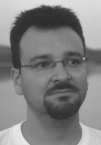
\includegraphics[width=1in,clip,keepaspectratio]{fig/fig_bio_guto.png}}
\noindent {\bf Antonio Augusto Fr�hlich}
received his Ph.D. in Computer Science from the Technical University of Berlin in 2001. He has been
a professor in the Computer Science Department, Federal University of Santa Catarina, Brazil
since 1995 and head of the Laboratory for Software and Hardware Integration since 2001. His current
research interests include embedded systems and operating systems.

\end{document}
